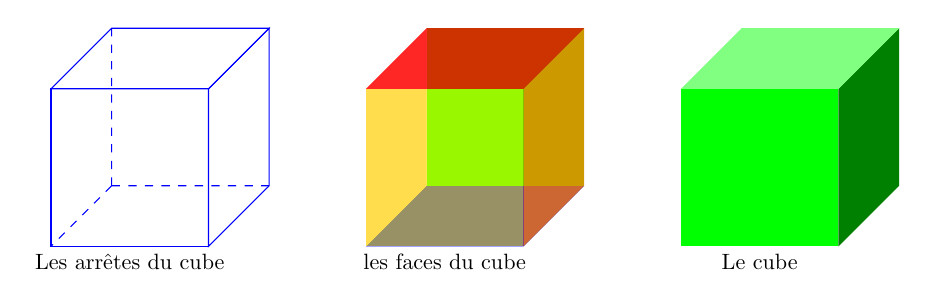
\begin{tikzpicture} 
\def \Width {2};
\def \Height {2};
\def \Depth {2};

%les arrêtes du cube
\begin{scope}
\def \translate {0};
\coordinate (O) at (0+\translate,0,0);
\coordinate (A) at (0+\translate,\Width,0);
\coordinate (B) at (0+\translate,\Width,\Height);
\coordinate (C) at (0+\translate,0,\Height);
\coordinate (D) at (\Depth+\translate,0,0);
\coordinate (E) at (\Depth+\translate,\Width,0);
\coordinate (F) at (\Depth+\translate,\Width,\Height);
\coordinate (G) at (\Depth+\translate,0,\Height);

\draw[dashed, blue] (O) -- (A) (O) -- (C) (O) -- (D);% arrêtes cachées
\draw[blue] (D) -- (E) -- (F) -- (G) -- cycle;% Right Face
\draw[blue] (C) -- (B) -- (F) -- (G) -- cycle;% Front Face
\draw[blue] (A) -- (B) -- (F) -- (E) -- cycle;% Top Face

\path (C)--(G) node[scale=0.8,midway,below]{Les arrêtes du cube};

%\node at (A) {A};
%\node at (B) {B};
%\node at (C) {C};
%\node at (D) {D};
%\node at (E) {E};
%\node at (F) {F};
%\node at (G) {G};
\end{scope}

%les faces du cubes
\begin{scope}
\def \translate {4};

\coordinate (O) at (0+\translate,0,0);
\coordinate (A) at (0+\translate,\Width,0);
\coordinate (B) at (0+\translate,\Width,\Height);
\coordinate (C) at (0+\translate,0,\Height);
\coordinate (D) at (\Depth+\translate,0,0);
\coordinate (E) at (\Depth+\translate,\Width,0);
\coordinate (F) at (\Depth+\translate,\Width,\Height);
\coordinate (G) at (\Depth+\translate,0,\Height);

\fill[blue] (O) -- (C) -- (G) -- (D) -- cycle;% Bottom Face
\fill[green] (O) -- (A) -- (E) -- (D) -- cycle;% Back Face
\fill[pink] (O) -- (A) -- (B) -- (C) -- cycle;% Left Face
\fill[orange,opacity=0.8] (D) -- (E) -- (F) -- (G) -- cycle;% Right Face
\fill[yellow,opacity=0.6] (C) -- (B) -- (F) -- (G) -- cycle;% Front Face
\fill[red,opacity=0.8] (A) -- (B) -- (F) -- (E) -- cycle;% Top Face


\path (C)--(G) node[scale=0.8,midway,below]{les faces du cube};
%\path (A)--(E) node[scale=0.8,midway,above]{solide (ou volume?)};

%\node at (A) {A};
%\node at (B) {B};
%\node at (C) {C};
%\node at (D) {D};
%\node at (E) {E};
%\node at (F) {F};
%\node at (G) {G};
\end{scope}

%le cube
\begin{scope}
\def \translate {8};

\coordinate (O) at (0+\translate,0,0);
\coordinate (A) at (0+\translate,\Width,0);
\coordinate (B) at (0+\translate,\Width,\Height);
\coordinate (C) at (0+\translate,0,\Height);
\coordinate (D) at (\Depth+\translate,0,0);
\coordinate (E) at (\Depth+\translate,\Width,0);
\coordinate (F) at (\Depth+\translate,\Width,\Height);
\coordinate (G) at (\Depth+\translate,0,\Height);

%\draw (O) -- (C) -- (G) -- (D) -- cycle;% Bottom Face
%\draw (O) -- (A) -- (E) -- (D) -- cycle;% Back Face
%\draw (O) -- (A) -- (B) -- (C) -- cycle;% Left Face
\fill[green!50!black] (D) -- (E) -- (F) -- (G) -- cycle;% Right Face
\fill[green] (C) -- (B) -- (F) -- (G) -- cycle;% Front Face
\fill[green!50!white] (A) -- (B) -- (F) -- (E) -- cycle;% Top Face


\path (C)--(G) node[scale=0.8,midway,below]{Le cube};
%\path (A)--(E) node[scale=0.8,midway,above]{solide (ou volume?)};

%\node at (A) {A};
%\node at (B) {B};
%\node at (C) {C};
%\node at (D) {D};
%\node at (E) {E};
%\node at (F) {F};
%\node at (G) {G};
\end{scope}


\end{tikzpicture}
